\documentclass[10pt,twocolumn]{article}
\usepackage{times}
\usepackage[pdftex]{graphicx}
\usepackage{algorithm}
\usepackage{algpseudocode}
\usepackage{qtree}
\graphicspath{{./}{figs/}}

\begin{document}
\title{Artificial Life Creation Comparing Genetic Algorithms And Genetic Programming}
\author{Tom Cammann\\\\
Computer Science, cy004947@reading.ac.uk}
\date{}
\maketitle
\begin{abstract}
This report focuses on the generating artificial life through two distinct methods, genetic algorithms and genetic programming. The report describes the fundamentals of these two methodologies, compares and contrasts their differences in the creation of similar artificial life. The report outlines tools developed during this project to accomplish an effective comparison of these two methods. These include a method of visualising the artificial life and the environment it inhabits during its existence. The outcome of this project demonstrates how genetic programming requires more advanced programming but can lead to novel and emergent behaviour, in contrast to genetic algorithms which are much simpler and can better replicate biological processes that go on around us. 
\end{abstract}


\section{INTRODUCTION}

Artificial life or ALife is the study and implementation of systems that are simulations or replications of natural life.
These systems can be biochemical, mechanical, computer software and many other medium that supports the existence of structured self controlled information.
This report will be looking at software artificial life, or Soft ALife and how it can be implemented using evolutionary computation.
Evolutionary computation has been used for the creation of artificial life for many decades, REF + EXAMPLE. Koza demonstrated the use of GP in 1992 ??? to solve the ant's nest problem. This used a set
of available commands for the ants to use, such as move forward, turn, move to nest. The idea was for
the ants problem was to order a set or resources on a simple 2D map. This simple example showed how ALife could
be used in the context of genetic programming.
Using evolutionary computation has many qualities that replicate naturally evolved life, and is one few computational methods known that can generate solutions to problems without human interaction.
Evolutionary computation has been applied to artificial life to generate life forms that can inhabit an environment and are 'solutions' to this environment.

\paragraph{}
Evolutionary computation generally works by generating a population of solutions to a problem, and then using this population to create a better next population that can solve the given problem better.
To create a better population crossover, mutation and selection are used in various forms to generate a fitter population.
Each of these populations is referred to as a generation.
Each member in the population is a solution to the problem, however these solutions do not have to be correct, and are often close to correct before many generations have passed.
Each member of the population is assigned a fitness value to correspond with how close the solution is to correct, or how effective the solution is.
In the Context of artificial life this fitness value may correspond to how well the life form survives in a given environment.

% why are we comparing these 2 methods
\paragraph{}
The purpose of this investigation is to compare and contrast the usage of genetic algorithms and genetic programming in the creation of artificial life. Genetic programming first became prevelvant in the early 1990 after Koza used used GP to solve ??? ~\cite{Koza90}. After the advancements made by Koza many applications for GP emerged and one of the earlier appications was in ALife. Before these advancements GA was the primary method for generating ALife.

However these two have very different implementations and usage, this report will investigate the usage of both in the context of artificial life creation. 
% Genetic programming can generate unique solutions, unrestrained, GA more restrained. 
Being able to compare this two types of algorithms will enable faster and better selection of algorithms during 
the design for an artificially evolved life form. It can be very daunting prospect to choose an algorithm
for developing and evolving aritificial life, there are many factors that will need to be considered and this
project will help future research into artificial life by comparing the two algorithms used in this project.
These algorithms will both have their benefits and pitfalls, with these exposed through this report this 
will enable better understanding of which algorithm to choose.


\paragraph{}
This project will design and implement an application which will launch and visualise the evolution of a
simple artificial life form. This application will make use of either genetic algorithms or genetic programming,
depending on conditions chosen. The initial parameters can be choosen for developing this artificial life form
and then this will produce a statistics of the evolutionary process, graphing the fitness over generations
and also the ability to visualise the life form in its environment. This will give the use the advantage of being
able to study the behaviour of the life form and understand it better than reading the genome of the fit life forms
produced by the evolutionary algorithm.


\paragraph{}
%how we compare them

\subsection{Requirements}
Comparing evolutionary algorithms in a fair and equal way has certain requirments. First both of the algorithms have to be implemented in such a way that allows a direct comparison. 
This can be done by constructing an enviromental problem for artificial life to solve, and then implemented a GA to solve to problem and then a GP to solve the problem. Direct
comparisons can be made on how these algorithms were implemented and how effecient and effective they are at solving the given enviromental proble. This problem can then be changed, 
and the algorithms reimplemented and a comparison can be made on how well the algorithms could be adapted to the new problem and again how effective the algorithms were at
finding a solution to this problem.

To setup these enviromental problems for the artificial life to solve an environment needs to be constructed, in which either algorithm can generate an artificial life form
to inhabit.

\paragraph{}
This interoperability between the two algorithms will also carry over to the visualisation of the artificial life. This will mean
that the visualisation and statistics generated about these artificial life forms will not care if the life form was created
through an GA or a GP, this information will be abstracted away. This will increase the ease of which the algoriths output can
be compared. However this will pose a challenge to program, to be able to implement the same functionality between the 
different algorithms. For example if the life form has a sight function or 'ability' this need to be programmed for both
the GA and GP because of the way the two algorithms work. These need give the same response in the same situation. One of the
algorithms can not have advantages over another.
	

\section{ANALYSIS}

\subsection{KEY PROBLEMS}
Producing artificial life that can solve the enviromental and situational problems that are presented in the simulated enviroment %TENSE?!
will be the biggest problem to over come in this project. Generating artificial life is a complex process; first an environment to simulate the artificial life has to be produced, and then
an interface between the artificial life and the environment has to be implemented. Finally the process for creating artificial life through a GA or GP can be produced, but these algorithms
both need to interface with the artificial life in an abstract manner so one can not distinguish between an GP implementation of artificial life and a GA implementation.

\paragraph{}
The first problem identified was producing an environment for the artificial life. This environment will support the artificial life and allow interaction between the resources present
in the environment and also other life in the environment. The environment that the artificial life will inhabit will be fairly simple with serveral parameters than can be affected such as
size, and objects for the artificial life to interact with. These objects that the artificial life can interact with will either be resources which the artificial life can possible consume
or an obstacle which the artificial life cannot move over, instead bypass. Keeping this environment simple will enable this project to focus more on producing a high quality artificial life
which will interact correctly and effectively with their environment. 

\paragraph{}
Another problem idenified is what methods and values would be used when comparing these two algorithms. To draw conclusions from this project the data generated from both algorithms needs 
to be comparable but also similar. Simple methods for comparing the algorithms will be runtime, memory/space requirments to compute a solution to a give problem. Further detail will need to
be drawn from the algorithms, such as average fitness of a whole generation of artificial life forms, the effectiveness of the algorithm to find a global optimimum solution and also the
intelligence of the artificial life produced. 

Producing these statistics will require the alorithms to be generating information that can be interpretted by a statistical model to be translated to graphs and values that can be
used to directly compare the algorithms. This will be done by implementing a several class that will aid this process, objects that can read in an entire generation of life forms
and record information about these life forms. 


The key issues with this project are based around a fair comparison of the algorithms. 

\section{GENETIC ALGORITHMS}

Genetic algorithms were first designed and implemented by ??? in ??? when ???.

The general form of a genetic algorithm uses genes to represent parameters inside a program.
These parameters effect the running of a program.
These genes were historically represented in binary form, however more modern implementations can use any value as a gene, from programming objects to double floating point numbers.
These genes must be able to mutate, this is easy to understand when using binary number, to mutate a binary number you flip one bit in the gene sequence. 

\begin{algorithm}
\caption{Pseduocode for a simple genetic algorithm}
\label{Genetic algorithm pseduocode}
\begin{algorithmic}
\Function{GenerateInitialPopulation}{$popsize$}
	\For{$i = 0 \to popsize$}
		\State $i \gets i + 1$ 
		\State \Return $popsize$
	\EndFor
\EndFunction

%\State $population =$ GenerateInitialPopulation()
%\State evaluate( $population )
%\Repeat
%\State $pop \gets 10$
%\State select fit individuals for crossover and/or elitism
%\State generate new individuals through crossover and mutation
%\State replace old generation with new individuals
%\State evaluate fitness of each individual in population
%\Until { fitest individual \geq fitness required OR time elapsed \geq time allowed } 
\end{algorithmic}
\end{algorithm}

\subsection{POPULATION REPRESENTATION}
In genetic algorithms each member of the population (or candidate solution) is represented by a list or string of values.
Each value represents a parameter that will be used in the solution.
The value could represent the number of iterations of a loop or represent a operator in a sum.
Traditionally binary numbers strings were used to represent a member of the population.
This was because of the ease of which this could be manipulated by computers and the simplicity mutations could be achieved.
To mutate a binary string a bit can be flipped.
This can work in most situations however it soon becomes apparent that this cannot useful in all situations.
%Fix and show formula? Find solutin.
If numbers are being represented in binary strings the most significant bit is at start of the string, if this is flipped then the number will change by a factor of ???.


\subsection{MUTATION}
In genetic algorithms mutation occurs on a per gene basis. If a mutation for a population member is needed then a gene in that~\cite{j1}. 

%better title needed!!!
%Section about how this project uses GA
\subsection{USAGE IN THIS}

\section{GENETIC PROGRAMMING}
%intro to gp
Genetic programming is one of the newest forms of evolutionary computing. 
%different ways


\subsection{POPULATION REPRESENTATION}

In genetic programming there is a variety of ways to represent a solution, however JGAP only supports one. Genetic algorithms are most
commonly represented in tree form and this is the only one supported by JGAP. Other methods of reprensenting a genetically programmed
solution such as a graph pose a greater programming/implementation challenge.
%TODO REF+SOURCE+EXAMPLE
The use of trees in genetic programming is easy to understand and was easy to use and implement for this project. In JGAP the tree
that represents the solution to the given problem is made up of genes, each gene represents a function which the life form can execute. 
This tree will contain only one root node and this node will be executed first, subsequent nodes can have a varying airity. The choice of
which node will be executed next will depend on the function node that was last executed. If the root node had an airity of two, then
the next node to execute will depend on the outcome of the root node. A simple example could be that the function checks whether the Y
position of the life form is greater than 50, if this is true it will execute the left node, if false it will execute the right node.
If in this example the position of the life form was greater than 50 on the Y-axis the left node would execute and this would 
execute its function, this could be move forward and then it would execute its subsequent node. Figure 1 shows how this could be
represented. What is hard to represent in the tree diagram is that fact that values can be passed down the tree during the execution.
In the execution of the example given in figure one, the amount that Y is greater than 50 would be passed down. This value can
then be used if input is needed. Some nodes will require input and other will not, this will depend on how they are setup during
development. 

%TREE
\begin{figure} [ht]
%\centering
\Tree [.{ $Y < 50$ } [.{Move Forward} {Turn Right} ] {\ldots} ]
\label{the-label-for-cross-referencing}
\caption{Example genetic programming execution tree}
\end{figure}


\subsection{MUTATION}
%asdsss

Mutation of the genetic program is handled by JGAP, however when and how much this mutation occurs can be altered through JGAP
configuration. The genetic code of each life form is made of of nodes on a tree, each of these nodes can be mutated by either
replacing the node or removing the node. The nodes can be replaced with an another node with the same airity and type, the
removal of node is fairly simple can is done by replacing the node with a null node. This will be a empty child node and
will just end execution if this node is reached during the trees execution.

\subsection{CROSSOVER}

As specified earlier this implementation is using trees, this means that the crossover during the evolutionary computation
will work through the tree representation. Using trees for representing your solution means that genetic cross over is
very simple. Two solution trees will first be selected for crossover, this selection will be based around the fitness of the given
solutions. This selection could be done 

\section{DEVELOPMENT}

This project was written in Java programming language and was developed on serveral operating systems during its life time. 
Java was chosen because of a strong prior intimate knowledge of the language and because of the libraries available to develop with. 
The evolutionary computation libraries which this project are based also use Java, this made interfacing with them very easy. 
Another reason Java was chosen was because of the graphical user interface programming libraries supplied as standard in Java. 
Having prior knowledge of these also meant that developing a visual format for the simulation could be accomplished.  Along with using 
Java for development several other tools were used these were Eclipse, Maven and Git. Eclipse is a Intergrated Development Enviroment or 
IDE which provides the user with an interface with faster programming and debugging ablities than are available as standard.
This meant faster development. Maven was used a build tool to manage dependcies and build jar files for running the application 
that contains the simulations. Using this made it easy to develop on any computer, as managing the depenecies necessary for the 
program done all by Maven. Git was used as the the version control system for this project, this was only adopted towards the 
end of the project as it became more necessary to manage versions and have a reliable branching system. This project was hosted 
on GitHub.com which meant that development could quickly begin from any location with git available. 

\subsection{DESIGN AND ARCHITECTURE}

Before implementation the architecture and design of this project was laidout in UML. The actual design has changed somewhat since the first UML diagram was
constructed, however this was expected and planned for. Most software projects usually have changing requirements and aims during their lifecycles as did this
project. The project used a software development cycle akin to agile software development, where first a feature list was made up with consolation, this list
contained all requirements for the upcoming sprint in the project. These features were then implemented in the project, such as developing new features in the
user interface. These features were then rigirously tested and fixed where necessary. Then the cycle was repeated again, drawing up a new feature list.
This project consisted 3 sprint periods where new features were drawn up, implemented, tested and bugs fixed.

As Java was the language being developed the design was very focused towards object orientation; this meant using the concepts of encapsulation, abstraction
and polymorphism. The map design revolved around encapsulating all life, resources and obstacles under one object, making this overall object only expose 
necessary attributes and readonly methods. This meant the underlying objects would not be distrubed by any GUI or user interface functions that exist on top.  

\subsection{PROJECT DESIGN}



\section{IMPLEMENTATION}
To evaluate a common artificial life form a simulation environment has been created.
This environment is a 2D arena where a life form must continue to consume food to survive, the more food the life form consumes the fitter the  

The underlying genetic and evolutionary computations were completed on a Java framework called JGAP (Java Genetic Algorithms Package).
This package provides a tried and very well tested method for using genetic algorithms in Java, while also providing the 
ability to extend the package and use the package to fit into this projects needs. The package was tested several times before usage
and simple life forms were developed to ensure this package was appropriate. Other packages such as %TODO other packages
were used but found to be lacking extendibility and documentation. JGAP has very good documentation, which meant that extending
the package and adapting the package to this projects needs was even easier.

JGAP provides two general over arching algorithm frameworks to work with, genetic algorithms and genetic programming. However
the package does not provide any high level interfaces between the genetic algorithms side and the genetic programming side. A 
lot of development during this project was focused on developing a framework for evolution that could incorporate both GAs and GPs developed
using JGAP. 

Visualising both the GP and GA in the life form meant developing an abstract way of representing the state of the life form. This was done
through an abstract class called ALife. This abstract class provided a high level interface for other objects to read (and modify if necessary)
the state of the life form. The abstract class contained many of the variables for the life form and the setting and getting functions 
associated with them. 

\subsection{LIFE}

This project has modeled life on upon a fairly simple scenario, with only a few state variables. The states that this life form
can control are: its position on the map, its orientation and its energy level. Its position can be changed by moving forward, these 
forms can only move in the direction they are facing. The can modify their orientation by moving either right or left of where they 
are currently facing. They can also change their energy, however this is more passive than active. The life form's energy will
deplete during its life based on how much it moves and what actions it takes. However its energy can be increased by consuming a 
resource, this resource will contain a number of calories which can be converted into energy. This conversion rate is variable
depending on the life forms parameters. 

The simulation is split up into frames, during each frame the life form has a chance to move and interact with the environment. If their
are multiple life forms in the environment then each life form in turn will get a chance to interact during this frame. These frames are
meant to represent time for the life forms, it has been slightly simplified to be an amount of time a life form can move forward or interact in another way. Only one 'major' interaction can be completed per frame. These include moving, consuming a resource and turning.

To survive in an environment the life form must keep its energy above zero for the duration of the simulation, if the life forms energy
drops to zero or below then the life form will be assumed deceased and can no longer make any more interactions with its environment. A simulation can have indefinite run time and how long the life form can survive will depend on its fitness and availability of resources for energy.

When a life form needs to be tested for fitness it is added to a map, and the life form is asked to make an action for every frame. The life form starts out
with a nominal energy value, so that it does not die at the start of the simulation. A fit life form will then make intelligent actions and move towards resources
that it can consume to increase its energy level. The fitness of the life forms is accessed usually assessed by its energy level at the end of the simulation. 


\subsection{MAP}

The environment that the life forms exist on during the simulations are referred to as maps. These maps are two dimensional and can vary in size.
The size of the map can be set at run time and can also be set to dynamically change during a run if necessary. The map also holds references
to the resources contained in the environment. The map is split up into cells which form a 2D grid for which the life forms can inhabite. 

Generally for evolving good fit life forms a unique map is generated for each simulation. This creates an enviroment in the life form has not
seen before and has not adapted to before. This means that the fit life forms are the ones which will be able to adapt to any give situation
and still be able to consume and interact with their environment. Each time a map is generated a new set of resources is generated with different
positions on the map and different calorie values. If a static map is used, with the same positions of resources for each run, a very specialised 
life form can evolve but as soon as this life form is transposed into another environment this life form is very unfit.

The resources generated for each map are randomly placed, with random calorific values. Only one resource can ocupy a cell on the map, each resoruce also has
a type which can be checked by the life form. If a life form is on top of a resource, i.e. if it is in the same cell then the life form can consume a resource. 
 

%talking about how the project framework
%how a frame to accommodate genetic programming and GA
\subsection{EVOLUTIONARY FRAMEWORK}
To investigate and compare these two algorithms %? algorithms??%
a framework to accommodate both algorithms was produced. This framework had to allow comparison of the effectiveness and fitness of the life forms evolved, efficency of the 
evolutionary computations in generating a fit life form and the correctness of the solutions generated. To enable all these things an abstract framework had 
to be developed to allow comparison without respect to the algorithm that was used. This first accomplished by visualising members of the population and 
manually inspecting the fitest life form of each generation. 


\subsection{VISUALISATION}
Visualisation of the solutions (or life forms) produced by the algorithms was key
to understanding the differences produced in the life forms between the two algorithms. A visualisation of the map and life form
was developed early on. The visualisation was developed using the model view controller architecture,
which meant that the map and the life form were completely detached from the visualisation.
The life form was made abstract by using an abstract class which contains the basic variables need for the life
form and some simple functions to get and set these variables. These include the life forms position, orientation
and energy level. The visualisation renders the 2D map with resources on, with the cell size depending on the attributes selected at runtime. The frame speed can
adjusted during the visualisation, but is default set to 5 frames per second. The visualisation itself is contained within the visualisation window. This window
provides access to the visualistation such as start, stopping and restarting the simualtion.


The visualisation has also been used to debug the life forms produced, to find errors in the project code which the life forms have ended up exploiting. An example
of this was during early development their existed a bug that cause the life form to stop decrementing its energy when it got to a map corner. When the simulation
was run with this bug in the life forms would evolve to find the corners of the map as they could get stuck their and never die. These life forms were not that fit 
as they usually only had a fitness value that was around their starting energy.

Later in development other features were added to the visulisation window. One of these features was the ability to import and export maps for the life forms to be
tested out on. A previously generated made could be loaded and the life form could be assessed on how it dealt with the that particular map. Producing this ablity meant that it would be easier to compare life forms, understanding exactly how they interacted with the same environment.
Another feature that was added was the ablitity to run the simulation frame by frame. The user can pause the simulation and step through the simulation, this again provides another method of fully understanding how a life form interacts with the enviroment. 
Along with the ablities to interact with the simulation was the ablitity to access information on the current life form, such as its genetic make what generation
and run time parameters were involved with its creation.

\subsection{PROGRAM FLOW}

\section{PROBLEMS ENCOUNTERED}

During implementation many hurdles had to be over come during each sprint phase of the project. However there were some issues that were much harder to overcome than others. One of these problems was
producing fair and equal output per time frame from each algorithm. The problem was that during each time frame the artificial life had the oppurtunity to survey its environment and then react to this
environment, hopefully in a way such that it can find more resources to consume, but the rules governing these interactions differed between the two algorithms.
This was because of the way the two algorithms generate output which controls the life form it was difficult to align
the rules governing the two algorithms. Originally the genetic programming solution controlled the artificial life by calling functions with in its chromosome tree, such as move forward, turn left etc.
However it was quickly realised that this would not work as the genetic program could call these functions multiple times during one time frame. This method would not work in this project because
of the way the genetic algorithm controls the artificial life. The GA did not have an opporutunity to call functions multiple times during one time frame. These methods of control had to be aligned. 

This was a difficult problem to solve, either the genetic algorithm had to modified in such a way that meant it could call interaction mehtods
a number of times or limit the number of calls the GP could make to these interactions. It was deemed easier to modify the GP, and a solution
was devised to fix this issue. The solution was to change the way the GP controlled the ALife. Instead of directly calling the interaction methods
the GP would instead return a number, this number would then refer to a specific action. The interactions that could take place in 
the environment are then hard coded into the program, e.g. if 1 is returned the ALife turns left, if 2 is returned the ALife turns right.

\paragraph{}
Another problem encountered was during refactoring of the code. Towards the end of the project the code base was fairly substantial, and any
untested modification to the code could produce errors. During some refactoring of the EnvironmentMap class serveral bugs slipped through
which meant a longer than necessary amount of time was spent debugging. However due to this project adopting the software version control system
Git, a 'diff' or file comparison could be made on the changed files. For the refactoring a new branch was created on git, the refactored code
was then developed on this refactoring branch, and the working unfactored code remained on the master branch. When the bugs occured in the
projects code the file comparsion between these two branches was extremely helpful in locating exactly what had been changed and what
possible bugs could have arisen from these changes. In this particular case a method that was acting as the sight for the artificial life
contained an erroneous 'not' symbol causing havoc. Initially it was hard to understand where the bug had arisen as many methods had been
altered, but using git diff meant I could easily inspect the changes and quickly went through any changes would could have produced the
results that were being produced by the project.

\section{RESULTS}

\section{TESTING}
The main goal behind testing this project was to ensure complete correctness of the implementation which utilises the JGAP framework.

Unit testing was one of the main tools used for this project. JUnit 4 was used in this project and was chosen for this project because
of its high renown in software engineering, and is usually the defacto choice for any testing in Java. It provides a robust framework
in which tests can be written and run with ease. JUnit also intergrates extremely well with Eclipse, the main IDE used during this project. Eclipse has default plugins for running and writing JUnit tests making the whole testing process even easier. Any test
failures will be shown, along with an exact reference on screen to where they failed. Individual test methods can then be run and
debugged to enable the code being test to be fixed very quickly.
This project also utilised Maven 3, Maven has the ablity to run JUnit tests and generate reports from these tests. Using the Maven
Surefire plugin and enabling reporting from these tests produced very useful reports on the project in HTML, although these were not
that useful as most of the tests were run through Eclipse. However Maven really comes into its own when other testing plugins are
utilised. This project used the Maven Cobertura plugin, Cobertura is a ''tool that calculates the percentage of code accessed by 
tests'' - http://cobertura.sourceforge.net. Using the Cobertura with Maven's reporting capabilities meant that detailed reports
on exactly what code was being tested by the unit tests. The HTML reports produced show the exact source code that is run during the
testing. This meant that JUnit tests could also be checked for correctness, and that any code that needed to be tested has not been
missed out.
Another tool used for testing was FindBugs, this tool usesd static code analysis to find errors in Java source code. This tool also
has a Maven reporting plugin which produced more HTML reports in readable and easily accessible format. Findbugs assisted in finding bugs in the projects code which would have otherwise been missed. FindBugs not only finds bugs and issues with the logic in the code
but also assess the performance, security, style and code convention. Many trivial issues can be raised by FindBugs such as 
incorrectly defining static fields or other simple programming mistakes. It can produce very useful feedback for producing
higher quality code and helps the programmer avoid common mistakes and improve efficientcy of the code. The find bugs report breaks
down the issues it finds by class, and then by priority. Most reports generated during this project contained many 'low' priority
issues such as: ''uses the same code for two switch clauses'', these issues are often ignored due to the fact they are artifacts
from code that is still in development, but occasionaly a 'high' prirority issue arises and these that often need to be immediately
addressed in the code. 

This project also used
CheckStyle for helping the code adhere to strict Java programming code conventions. Adhereing to these code conventions meant that
the code produced is more readable, easier to understand, easier to debug and helps avoid bugs.

This complete strategy for testing was chosen as it enabled this project to focus on development of the code and spend as little
time as possible on developing tests. This streamlined testing process improved the efficenency of the project, tests could 
be written, tested and verified in very little time. Using Cobertura the tests could be verified that they were covering the
correct areas, FinbBugs, Checkstyle improved the readablity and transparency of the code and also helped stop static code
bugs occur.


\paragraph{}

The Unit tests written for this project were aimed at the most important and complex areas of code. Exhaustive testing was 
unfortuantely of the scope of this project, and full test coverage of the entire code was not feasible to implement.

This project focused on implementing test driven development, TDD, which meant writing unit tests alongside writing project code.
This increased the work load but was essential to ensure correctness of the code being produced. Major benefits were seen from
writing these unit tests concurently with the project code. Bugs that would have very hard to track down from a mis-assigned
variable were very easy to locate. Performance of the code was also improved, due the fact that each time JUnit runs the test
it also reports how long this took. Using this it was easy to see which parts of the code are very innefficent and which needed
refactoring. 

However the 
areas of the code that could produce 'silent' bugs were targeted for testing. A silent bug is one which would not throw an error
or even produce erroreous output, but would perhaps alter the outcome of a run slightly. A example of this was a method that
was used as the eyes of the ALife in the genetic algorithm. The range value is taken from the set of genes, and is used to 
to limit how far the artificial life can see. The method that was written accidentaly reduced this range by 1 due to an issue
in incrementing a for-loop. This bug was not spotted until a test for this method was written. 
\paragraph{}

The logging used in this project was implemented through Log4j, this system enabled this project to customise the logging 
ablitity without costing the project runtime. During debugging the trace log can be enabled which will slow down the
run time of the project but provide invaluable help when debugging the code. When logging is turned off the perfomance
of the code has very similar performance to code with any logging statements in, this makes log4j very powerful. Also
log4j has many built in output and format options which means one can customise it to suit any project. Log4j is often
thought of as industry defacto logging platform and therefore is highly supported meaning increased performance
and one of the safest logging platforms in terms of the number of bugs because of its age and community support. All these
factors contribute to a highly effective and stable logging platform. 

Log4j has several levels of logging, fatal, error, warn, info, debug, trace. Each of these logging levels can be used throughout
the project, however logging in this project was used with a strict set of rules. Any errors or errorneous outcomes will 
be logged as either fatal or with error level logging, fatal will be used in a case where any further outcome of the project
will be invalid or erroroneous, error will be used for logging any error that will cause the current run of the system to be
erroroneous however will probably not impact the rest of the run. Warn will be used when parameters exceed recommended
extremes or an acceptable or expected bad input is recorded and adjusted. Info is used for recording the current state of
the projec run, for example each time a new generation is started during either the GA or GP run the info logging level is
used to print and record that this is the current state of the program. It is used to record high level state of the run,
not the low level state of each of the components which combine together during this run. Other common info level logging
information would be the fitness of the entire generation or if a target is reached in the code such as a fitness leve.
Debug and trace are only used for debugging, and often trace is disabled at run time because of the impact enabling this
logging level has on the code. Most logging that occurs in this project is trace or debug logging, logging statements are
put into frequently used methods and classes to record the current state that they are in and to help during the debugging
process. The trace log level is used for calls that are very frequent and if not disabled would likely produce a significant
low down during runtime. 

\subsection{Test ALife}

Testing the correctness of the ALife was a slightly more complex task, and could not be completely automated through unit testing.
The common errors that occured during development of the project which affected the ALife simulation were normally due to the
artificial life evolving to exploit bugs in the simulation. One such bug allowed to the artificial life to never die by exploiting
a case were it could skip code that required energy to drecremented at the end of each turn, and therefore the ALife did not need
to consume resources to become fit.

Another common bug would be where the ALife would get stuck in the corner of the map and not be able to escape this corner. This
was an error to do with the ALife's navigation and movement commands.

These bugs were discovered by inspection and not through automated testing. This meant these bugs took longer to find and longer to
debug. Automated tests could not be written for the ALife as there was not an expected behaviour to test against. The best
test for these artificial life forms was the fitness function. The life form would be successful and pass the tests if the fitness
was above a certain threshold. Through a particular run of the project if the fitness outcomes were expectionally high or close to 
zero then this run would probably have a bug in the implementation of the project and would be inspected. When this occured
it was often a time costly bug as the cause would not be given and would have to be found. However the tools developed in this
project helped greatly in finding these bugs. The first one was using the visualisation frame, an ALife form could be chosen
and run on a chosen map. The artificial life could then be debugged by stepping through its life, using the visualisation tools.
Using the verbose logging setup throughout the project and the ability to run the life form time frame by time frame meant that
some bugs could quickly be found through this process. Different maps could be loaded and the whole process reloaded again for
repeatitive testing. 


\subsection{TESTING THE ENVIRONMENT}


\begin{figure} [ht]
\centering
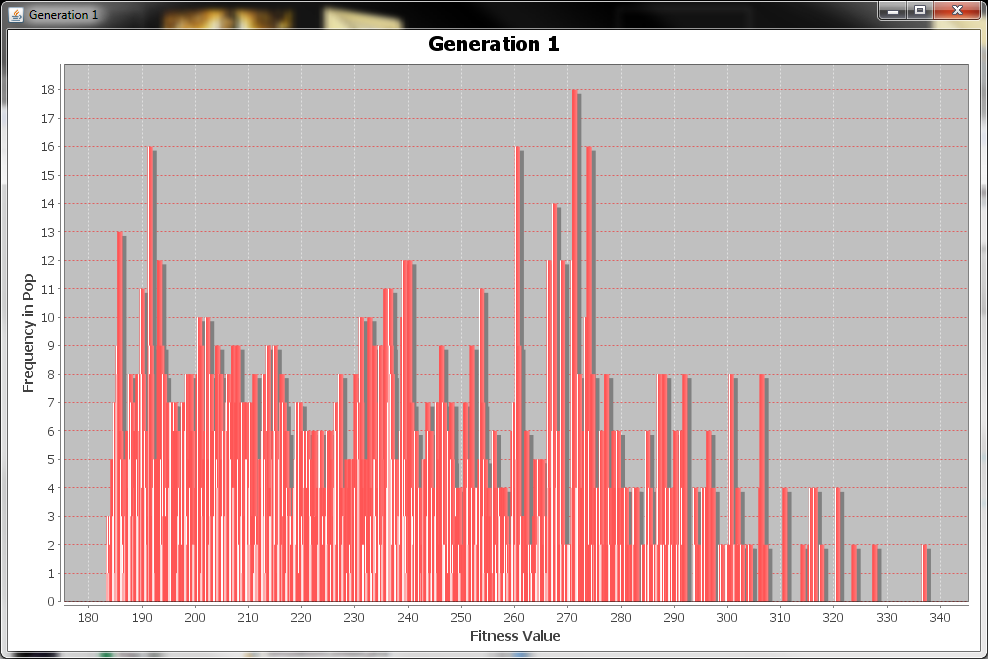
\includegraphics[scale = 0.25]{gen1-2500.png}
\caption{My figure}
\label{the-label-for-cross-referencing}
\end{figure}


\bibliographystyle{plain}
\bibliography{disseration}

\end{document}
